\documentclass[12pt,]{article}
\usepackage{lmodern}
\usepackage{amssymb,amsmath}
\usepackage{ifxetex,ifluatex}
\usepackage{fixltx2e} % provides \textsubscript
\ifnum 0\ifxetex 1\fi\ifluatex 1\fi=0 % if pdftex
  \usepackage[T1]{fontenc}
  \usepackage[utf8]{inputenc}
\else % if luatex or xelatex
  \ifxetex
    \usepackage{mathspec}
  \else
    \usepackage{fontspec}
  \fi
  \defaultfontfeatures{Ligatures=TeX,Scale=MatchLowercase}
\fi
% use upquote if available, for straight quotes in verbatim environments
\IfFileExists{upquote.sty}{\usepackage{upquote}}{}
% use microtype if available
\IfFileExists{microtype.sty}{%
\usepackage{microtype}
\UseMicrotypeSet[protrusion]{basicmath} % disable protrusion for tt fonts
}{}
\usepackage[margin=1in]{geometry}
\usepackage{hyperref}
\hypersetup{unicode=true,
            pdftitle={Displacement of fishing effort by Large Scale Marine Protected Areas},
            pdfborder={0 0 0},
            breaklinks=true}
\urlstyle{same}  % don't use monospace font for urls
\usepackage{natbib}
\bibliographystyle{plainnat}
\usepackage{longtable,booktabs}
\usepackage{graphicx,grffile}
\makeatletter
\def\maxwidth{\ifdim\Gin@nat@width>\linewidth\linewidth\else\Gin@nat@width\fi}
\def\maxheight{\ifdim\Gin@nat@height>\textheight\textheight\else\Gin@nat@height\fi}
\makeatother
% Scale images if necessary, so that they will not overflow the page
% margins by default, and it is still possible to overwrite the defaults
% using explicit options in \includegraphics[width, height, ...]{}
\setkeys{Gin}{width=\maxwidth,height=\maxheight,keepaspectratio}
\IfFileExists{parskip.sty}{%
\usepackage{parskip}
}{% else
\setlength{\parindent}{0pt}
\setlength{\parskip}{6pt plus 2pt minus 1pt}
}
\setlength{\emergencystretch}{3em}  % prevent overfull lines
\providecommand{\tightlist}{%
  \setlength{\itemsep}{0pt}\setlength{\parskip}{0pt}}
\setcounter{secnumdepth}{0}
% Redefines (sub)paragraphs to behave more like sections
\ifx\paragraph\undefined\else
\let\oldparagraph\paragraph
\renewcommand{\paragraph}[1]{\oldparagraph{#1}\mbox{}}
\fi
\ifx\subparagraph\undefined\else
\let\oldsubparagraph\subparagraph
\renewcommand{\subparagraph}[1]{\oldsubparagraph{#1}\mbox{}}
\fi

%%% Use protect on footnotes to avoid problems with footnotes in titles
\let\rmarkdownfootnote\footnote%
\def\footnote{\protect\rmarkdownfootnote}

%%% Change title format to be more compact
\usepackage{titling}

% Create subtitle command for use in maketitle
\newcommand{\subtitle}[1]{
  \posttitle{
    \begin{center}\large#1\end{center}
    }
}

\setlength{\droptitle}{-2em}

  \title{Displacement of fishing effort by Large Scale Marine Protected Areas}
    \pretitle{\vspace{\droptitle}\centering\huge}
  \posttitle{\par}
  \subtitle{Updated on 2018-09-29}
  \author{Juan Carlos Villaseñor-Derbez\textsuperscript{1} John
Lynham\textsuperscript{2}}
    \preauthor{\centering\large\emph}
  \postauthor{\par}
      \predate{\centering\large\emph}
  \postdate{\par}
    \date{\textsuperscript{1}Bren School of Environmental Science and Management,
University of California Santa Barbara, Santa Barbara,
CA\newline\textsuperscript{2}Department of Economics, University of
Hawaii at Manoa, Honolulu, HI}

\usepackage{float}
\floatplacement{figure}{H}
\usepackage{lineno}
\linenumbers

\begin{document}
\maketitle
\begin{abstract}
Large-scale Marine Protected Areas (LSMPAs) have seen a significant
increase over the last years. Fishing effort is effectively eliminated
within these protected areas upon implementation. The benefits of
reducing effort have been largely studied, and include increases in
abundance, biomass, and diversity within the bounded regions. These
no-take zones may produce spillover effects, which provide fish for
outside areas. However, the economic and ecological implications of
displacing fishing effort are not yet fully understood. Novel data
products that track fishing effort at the vessel-level allow us to
identify changes in fleet- and vessel-level behavior upon the
implementation of protected areas, as well as how these redistribute.
This papers evaluates the implications of implementing LSMPA, by
evaluating changes in fishing hours, showing that vessels in the
effected region reduce fishing effort after the implementation of PIPA.
Our results are robust to a set of specifications. We also track the
relative spatial allocation of fishing events thorugh time, and identify
that areas closer to PIPA show an increase in relative fishing hourse
due to the displacement of PIPA-fishing vessels. Our results not only
provide an impact evaluation of the effect of LSMPAs on fishing
activity, but provide insights into vessel redistribution dynamics,
which may have ecological and economic implications.
\end{abstract}

\section{Introduction}\label{introduction}

Marine Protected Areas (MPAs) are intended to safeguard parts of the
ocean from extractive activities such as fishing. Current international
goals aim to ``effectively protect 10\% of the ocean environments by
2020''. In an effort to meet this target, the world has seen a rapid
increase in MPA coverage \citep{wood_2008,sala_2018b}. A significant
part of this rapid increase can be attributed to the designation of a
small number of Large Scale Marine Protected Areas {[}LSMPAs;
\citep{gray_2017}{]}. These are defined as MPAS with at least 250,000
km\textsuperscript{2} \citep{toonen_2013} in extension, and are often
implemented in the pelagic environment, where the dominant human
activity is industrial fishing \citep{gray_2017}.

Due to weak property rights, limited habitat transformation, and
potentially lower management costs, pelagic MPAs provide a great
opportunity to safeguard the oceans \citet{game_2009}{[}\^{}d{]}. A
growing body of literature has also shown that closing the high seas to
all fishing -effectively, turning them into a LSMPA- could increase
fishery yields and profitability of fisheries, without negligible costs
to food security
\citep{white_2014,sumaila_2015,sala_2018,schiller_2018}. However, as
with customary MPAs, it is important that we understand the
socioeconomic implications of management interventions.

Given the relatively recent establishment of most LSMPAs, very little is
known about their human dimensions and implication for fisheries
\citep{gray_2017}. LSMPAs were erroneously assumed to have little social
implications due to their remoteness \citep{agardy_2011,gray_2017}.
However, the anticipation of a LSMPA can lead to preemptive overfishing,
which can erode or delay the expected benefits of the intervention
\citep{mcdermott_2018}. LSMPAs have received great attention in terms of
governance and enforcement, but are yet to be the focus of economic
analyses \citep{gray_2017}. For example, \citet{mcdermott_2018} show
that fishing effort within the Phoenix Islands Marine Protected Area
(PIPA) is effectively reduced after implementation, and describe changes
in fishing behavior pre-implementation. \citet{cabral_2017} analyse the
redistribution of fishing and non-fishing vessels following the
implementation of MPAs in California, and find that responses are
idiosyncratic; commercial dive boats follow a fishing-the-line pattern,
while some fishing boats follow an ideal free distribution. The way in
which fishers react to a spatial closure can have major implications in
its outcome \citep{hilborn_2006,krueck_2017,viana_2017}. This highlights
the need to understand how fishers react to the implementation of a
LSMPA, and fishing effort changes and is spatially redistributed.

The main objective of this paper is to identify how fishers adapt to the
implementation of LSMPAs. We combine novel vessel tracking technologies
and causal inference techniques to identify behavioral changes of
fishing vessels due to the implementation of PIPA. We focus on fishing
hours and distance traveled as outcome variables that fishers might
adjust following implementation of a LSMPA in an impact-evaluation
fashion. Additionally, we evaluate the spatial redistribution of fishing
effort that existed within PIPA before its implementation. This work
provides novel empirical insights into fisher's responses to the
implementation of LSMPAs, and can help guide future interventions.

\section{Methods}\label{methods}

This section is divided into two main parts. First, we provide a general
description of AIS data and the process of identification of
vessel-level fishing events done by Global Fishing Watch\footnote{Global
  Fishing Watch: \url{globalfishingwatch.org}}. Alongside, we describe
the subset of data that we use for these analyses. When relevant, we
also point out possible shortcomings in the data, or factors that must
be considered in the later analyses. We then move on to explain our
empirical strategy for the identification of the behavioral changes and
redistribution of fishing effort.

\subsection{Data}\label{data}

Automatic Identification Systems are on-board devices intended to
provide at-sea safety and prevent ship collisions by broadcasting vessel
position, course, and activities to surrounding vessels. These
broadcasted messages can be received by satellites and land-based
antennas. GFW uses a neural network to infer vessel characteristics and
whether each broadcasted position represents a fishing event, thus
allowing us to estimate near real-time fishing events globally since
2012 \citep{kroodsma_2018}. Our data contain information for 2012 -
2017. The recent addition of satellites that can receive AIS signals
causes an apparent increase in the number of broadcasted AIS messages
(\emph{i.e.} points), and therefore number of vessels and fishing hours.
The variability in AIS data and ocean conditions require that temporal
trends be taken into account. We do that by obtaining a subset of data
that meet a BACI design, which gives us the full tracks for vessels
affected and unaffected by the implementation of PIPA.

Our data contain over 45 million individual AIS messages (\emph{i.e.}
positions) for 371 purse seiners and longliners. A total of 233 vessels
have fished within PIPA waters; 217 did so at least once before 2015.
However, not all vessels continued to fish elsewhere after PIPA
implementation: 34 vessels have no recorded AIS messages after
2015\footnote{The 34 missing vessels might have exited the fishery, been
  decommissioned or sold (therefore changing their AIS and mmsi), or
  turned off their AIS transmitters. In either case, we are not able to
  observe these.}, leaving us with 183 vessels that fished inside PIPA
before its implementation, and continued to fish elsewhere afterward.
New vessels might have also entered the fishery after PIPA closure, and
were likely not exposed to the policy intervention in the pre-treatment
period. To account for this, we identify a subset of vessels which we
track since before the implementation of PIPA, and categorize them as
treated or control vessels. Our treatment and control groups are defined
as follows.

The treatment group contains all vessels (n = 183) that fished within
PIPA at least once before the closure, and that continued to fish
elsewhere afterwards. Vessels in the control group meet all three of the
following conditions: i) vessels never fished within PIPA waters, ii)
vessels belong to other PNA countries, and iii) vessels have fished in
surrounding areas (\emph{i.e.} PNA-countries' EEZ) before and after PIPA
closure. For each vessel meeting these characteristics, we calculate
their total monthly fishing hours. Figure \ref{fig:baci_strict} provides
a visual representation of the vessel-level fishing events that make up
each group through time. Table \ref{tab:baci_n_s} shows the number of
vessels following a BACI design, as well as the fishing hours, before
and after PIPA.

\begin{figure}
\centering
\includegraphics{C:/Users/JC/Documents/GitHub/MPA_displacement/docs/Manuscript_files/figure-latex/unnamed-chunk-4-1.pdf}
\caption{\label{fig:unnamed-chunk-4}\label{fig:baci_strict}Stream of fishing
events by vessels through time. Each line represents a vessel, with dots
indicating months with fishing activity and colors indicating the pre
and post periods.}
\end{figure}

\begin{table}[H]

\caption{\label{tab:unnamed-chunk-5}\label{tab:baci_n_s}Number of fishing vessels and fishing hours by gear and treatment group before and after PIPA.}
\centering
\begin{tabular}[t]{llrrrr}
\toprule
Gear & Treatment & n & Before & After & Change (A / B)\\
\midrule
drifting\_longlines & FALSE & 85 & 474.47780 & 462.5491 & 0.9748593\\
drifting\_longlines & TRUE & 115 & 544.61935 & 522.8392 & 0.9600085\\
purse\_seines & FALSE & 36 & 59.49026 & 154.5776 & 2.5983673\\
purse\_seines & TRUE & 68 & 52.91534 & 131.5452 & 2.4859561\\
\bottomrule
\end{tabular}
\end{table}

\clearpage

\subsection{Analysis}\label{analysis}

The first analysis focuses on identifying the response of fishing
vessels to PIPA closure. Our variables of interests are fishing effort,
indicated by total fishing hours per month, and distance traveled (Km)
on every fishing trip. We compare fishing hours\footnote{And soon,
  distance} before and after the implementation of PIPA using a
Difference-in-Differences approach, where we track the variable of
interest for vessels that used to fish inside PIPA and vessels that
never fished inside PIPA, before and after PIPA implementation. Our
specification is the following:

\[
y_{i,t} = \alpha + \beta_1 Post_t + \beta_2 Treat_i + \beta_3 Post_t \times Treat_i + \mu_1Y_t + \mu_2Y_t^2 + \phi_t + \gamma_i + \epsilon_{i,t}
\]

Where \(y_{i,t}\) is the variable of interest for vessel \(i\) in time
period \(t\). A dummy variable \(Post_t\) takes the value of 0 for all
dates prior to PIPA implementation and a value of 1 for all dates
including and following PIPA implementation. \(Treat_i\) is a dummy
variable indicating whether a vessel belongs to the control
(\(Treat_i = 0\)) or treatment (\(Treat_i = 1\)) group. \(\alpha\) is
the standard intercept, \(\beta_1\) captures the temporal trend change,
\(\beta_2\) captures the difference between treated and control groups,
and \(\beta_3\) is our parameter of interest: de DiD estimate capturing
the treatment effect. Finally, \(\mu_1\) and \(\mu_2\) are coefficients
for a second order polynomial for years (\(Y_t\)), while \(\phi_t\) and
\(\gamma_i\) represent month-, and flag-level dummies that account for
seasonality or country-level management interventions\footnote{An
  earlier specification included years as a dummy variable. Such results
  are included in the appendix, but are similar to the ones found under
  current specification.}.

Our second part of the analyses focuses on the redistribution of fishing
effort. In other words, identifying where do vessels that used to fish
inside PIPA go after its establishment. We calculate the monthly
relative distribution of fishing hours by all treated vessels across all
fished EEZs and the high seas. These trends are shown in Figure
\ref{fig:redist_trend_ps}, and the relative temporal change is presented
in Table \ref{tab:ba_disp}. EEZs that had sporadic fishing events were
pooled into a group of ``others'', leaving us with a total of n = 12 and
n = 10\footnote{This number is likely to change upon finalizing the
  spatial analysis of longliners, which is currently running.} spatially
defined regions (\emph{i.e.} EEZs, High Seas, ``other EEZs'', and PIPA)
for purse seiners and longliners, respectively.

To evaluate this change in effort allocation, we regress our variable of
interest (\emph{i.e.}fishing hours) on the interaction between a dummy
variable indicating the policy intervention and a dummy variable for
countries. This gives us the by-country change in proportional
allocation of fishing effort:

\[
y_{i,t} = \alpha + \beta_1Post_t + \beta_{2,i}Country_i + \beta_{3,i}Post_t \times Country_i + \epsilon_{i,t}
\]

Our variable of interest, \(y_{i,t}\) represents the proportion of
fishing hours that country \(i\) receives at time \(t\). \(Post\) also
represents a policy dummy that takes the value of 0 for all dates before
implementation of PIPA, and 1 otherwise. \(Country\) is a dummy variable
for countries, interpreted as individual EEZs, the high seas, and a
group of ``other EEZs''. Our parameter of interest is \(\beta_{3,i}\),
which captures the country-level change in proportional fishing effort.

All regression coefficients were estimated via ordinary least squares,
and heteroskedastic-robust standard errors were calculated. All analyses
were performed in R version 3.5.1 \citep{rcore_2018}. Raw data and code
used in this work are available on
\href{https://github.com/jcvdav/MPA_displacement}{github}.

\begin{table}[H]

\caption{\label{tab:unnamed-chunk-8}\label{tab:ba_disp}Changes in the relative allocation of fishing effort by region (EEZ, PIPA, high seas) and gear.}
\centering
\begin{tabular}[t]{lrr}
\toprule
country & Longliners & Purse seiners\\
\midrule
PIPA & -11.48 & -8.54\\
KIR & 1.28 & 2.76\\
HS & 0.00 & 0.00\\
COK & 0.00 & 0.34\\
FSM & 0.00 & 0.55\\
\addlinespace
MHL & NA & -0.55\\
NRU & 0.00 & 0.16\\
PNG & 0.00 & -10.02\\
SLB & -8.48 & 2.13\\
TKL & NA & 0.19\\
\addlinespace
TUV & 7.23 & 1.47\\
others & 22.55 & 11.51\\
\bottomrule
\end{tabular}
\end{table}

\clearpage

\section{Results}\label{results}

Our data suggest that purse seiners and longliners have different
responses to the implementation of a Large-Scale Marine Protected Areas.
Fig. \ref{fig:all_vessels} shows that mean fishing hours for purse
seiners have an abrupt increase, just before January 1st, 2015. This
trend is observed for both treated and control groups. The pattern
closely corresponds with the increase in total hours, but the total
number of vessels doesn't entirely follow this pattern. The increase in
fishing hours might be caused by the increased number of
satellites\footnote{Need to check this. Not sure any satellites were
  incorporated during 2014. It is also possible that PNA countries
  started enforcing the requirement of having an AIS unit. On either
  case, both treatment and control groups seem to be affected equally.}.
Longliners, however, show no apparent trend with a clear seasonality
\citep{ortuocrespo_2018}. The number of mmsi codes also increases
slightly through time, but becomes stable after 2015. For both gears and
across all measures, the treatment and control vessels follow similar
patterns, confirming our claim that the control group provides a
plausible counterfactual.

\begin{figure}
\centering
\includegraphics{C:/Users/JC/Documents/GitHub/MPA_displacement/docs/Manuscript_files/figure-latex/unnamed-chunk-9-1.pdf}
\caption{\label{fig:unnamed-chunk-9}\label{fig:all_vessels}Fishing hours and
number of vessels by month for all vessels. Vertical dashed line
indicates PIPA closure.}
\end{figure}

Our DiD analysis shows that treated purse seiners reduce their fishing
effort after PIPA implementation in the order of 16 hours per month.
This result is robust and significant (\emph{p \textless{} 0.05}) for
all model specifications, with the effect varying between
\(\beta_3 = -16.457\) and \(\beta_3 = -18.709\). Model specifications
that include the year polynomial show lower values for the \(\beta_1\)
coefficient associated to the \(Post_t\) policy dummy, and show positive
and negative values for \(\mu_1\) and \(\mu_2\), the linear and
quadratic terms for \(Y_t\), respectively. These effectively represent
the patterns observed in Figure \ref{fig:all_vessels}.

Longliners show a similar pattern of effort reduction. However, the
magnitude of the \(\beta_3\) coefficient is smaller (ranging from
\(\beta_3 = -9.851\) to \(\beta_3 = -14.850\)) and not significant
across all model specifications. This, along with higher standard error
values suggest that longliners have a smaller and more variable response
to the implementation of LSMPAs.

Regressions coefficients for each gear type are shown in Tables
\ref{tab:purse} and \ref{tab:long}. Column (1) presents the DiD
regression with no fixed effects, column (2) includes month fixed
effects, column (3) includes month and the second degree polynomial for
years, and column (4) includes all of the above and country-level fixed
effects.

\begin{table}[!htbp] \centering 
  \caption{\label{tab:purse}Fishing hours from GFW for purse seiners (n = 106; 38 control, 68 treatment). Asterisks indicate significance levels. Numbers in parenthesis represent heteroskedastic-robust standard errors.} 
  \label{} 
\begin{tabular}{@{\extracolsep{5pt}}lcccc} 
\\[-1.8ex]\hline 
\hline \\[-1.8ex] 
 & \multicolumn{4}{c}{\textit{Dependent variable:}} \\ 
\cline{2-5} 
\\[-1.8ex] & \multicolumn{4}{c}{hours} \\ 
\\[-1.8ex] & (1) & (2) & (3) & (4)\\ 
\hline \\[-1.8ex] 
 post & 95.087$^{***}$ & 99.232$^{***}$ & 38.349$^{***}$ & 41.920$^{***}$ \\ 
  & (5.877) & (5.453) & (7.423) & (8.214) \\ 
  & & & & \\ 
 treated & $-$6.575 & $-$5.597 & $-$3.811 & 6.541 \\ 
  & (4.985) & (4.564) & (4.247) & (5.195) \\ 
  & & & & \\ 
 year &  &  & 12,828.900$^{***}$ & 16,665.590$^{***}$ \\ 
  &  &  & (2,451.444) & (3,717.658) \\ 
  & & & & \\ 
 year2 &  &  & $-$3.178$^{***}$ & $-$4.131$^{***}$ \\ 
  &  &  & (0.609) & (0.923) \\ 
  & & & & \\ 
 post:treated & $-$16.457$^{**}$ & $-$16.739$^{***}$ & $-$17.304$^{***}$ & $-$18.709$^{***}$ \\ 
  & (6.856) & (6.460) & (6.254) & (6.787) \\ 
  & & & & \\ 
 Constant & 59.490$^{***}$ & 65.485$^{***}$ & $-$12,946,334.000$^{***}$ & $-$16,807,078.000$^{***}$ \\ 
  & (4.422) & (6.132) & (2,473,372.000) & (3,759,572.000) \\ 
  & & & & \\ 
\hline \\[-1.8ex] 
Month FE & No & Yes & Yes & Yes \\ 
Flag FE & No & No & No & Yes \\ 
Observations & 3,867 & 3,867 & 3,867 & 3,481 \\ 
R$^{2}$ & 0.171 & 0.243 & 0.281 & 0.299 \\ 
\hline 
\hline \\[-1.8ex] 
\textit{Note:}  & \multicolumn{4}{r}{$^{*}$p$<$0.1; $^{**}$p$<$0.05; $^{***}$p$<$0.01} \\ 
\end{tabular} 
\end{table}

\begin{table}[!htbp] \centering 
  \caption{\label{tab:long}Fishing hours from GFW for longliners (n = 203; 88 control, 115 treatment). Asterisks indicate significance levels. Numbers in parenthesis represent heteroskedastic-robust standard errors.} 
  \label{} 
\begin{tabular}{@{\extracolsep{5pt}}lcccc} 
\\[-1.8ex]\hline 
\hline \\[-1.8ex] 
 & \multicolumn{4}{c}{\textit{Dependent variable:}} \\ 
\cline{2-5} 
\\[-1.8ex] & \multicolumn{4}{c}{hours} \\ 
\\[-1.8ex] & (1) & (2) & (3) & (4)\\ 
\hline \\[-1.8ex] 
 post & $-$11.929 & $-$6.968 & $-$15.550 & $-$6.761 \\ 
  & (7.969) & (7.975) & (10.181) & (11.289) \\ 
  & & & & \\ 
 treated & 70.142$^{***}$ & 72.314$^{***}$ & 71.985$^{***}$ & 14.026$^{*}$ \\ 
  & (7.200) & (7.200) & (7.279) & (7.988) \\ 
  & & & & \\ 
 year &  &  & $-$6,673.971$^{*}$ & 21,188.090$^{***}$ \\ 
  &  &  & (3,606.793) & (5,631.642) \\ 
  & & & & \\ 
 year2 &  &  & 1.657$^{*}$ & $-$5.259$^{***}$ \\ 
  &  &  & (0.894) & (1.398) \\ 
  & & & & \\ 
 post:treated & $-$9.851 & $-$12.290 & $-$12.779 & $-$14.850 \\ 
  & (9.294) & (9.262) & (9.334) & (9.563) \\ 
  & & & & \\ 
 Constant & 474.478$^{***}$ & 449.960$^{***}$ & 6,719,355.000$^{*}$ & $-$21,341,371.000$^{***}$ \\ 
  & (6.328) & (9.440) & (3,633,994.000) & (5,644,837.000) \\ 
  & & & & \\ 
\hline \\[-1.8ex] 
Month FE & No & Yes & Yes & Yes \\ 
Flag FE & No & No & No & Yes \\ 
Observations & 9,460 & 9,460 & 9,460 & 8,269 \\ 
R$^{2}$ & 0.027 & 0.041 & 0.042 & 0.094 \\ 
\hline 
\hline \\[-1.8ex] 
\textit{Note:}  & \multicolumn{4}{r}{$^{*}$p$<$0.1; $^{**}$p$<$0.05; $^{***}$p$<$0.01} \\ 
\end{tabular} 
\end{table}

Recall that to evaluate the redistribution of fishing effort we only
track fishing vessels that belong to the treated group. In this case, we
calculate the proportion of fishing effort allocated every month to each
spatially explicit region outlined by EEZs and the high seas. For purse
seiners, these represent 9 main EEZs, PIPA, the high seas, and a group
of other EEZs. Figure \ref{fig:redist_trend_ps} shows the monthly
relative fishing hours that each region received by all 183 treated
vessels. The top-left panel shows the change in fishing effort inside
PIPA, including the preemptive fishing and immediate reduction
previously reported \citep{mcdermott_2018}.

The change in the relative allocation of fishing effort by purse seiners
increases in eight of the 12 regions after PIPA implementation (Table
\ref{tab:disp_mod}). The largest increase is observed for the I-Kiribati
EEZ, with an average increase of 0.11 (\emph{p \textless{} 0.001}). In
other words, the redistribution of treated vessels caused a 10\%
increase in the \emph{relative} allocation of fishing effort within
I-Kiribati waters. The only decrease is observed for Papua New Guinea,
but the coefficient is not significant. Figure \ref{fig:map_change_ps}
provides a spatial representation of these changes. It is evident that
the increase in relative fishing effort is greater for for regions
closer to PIPA.

\begin{figure}
\centering
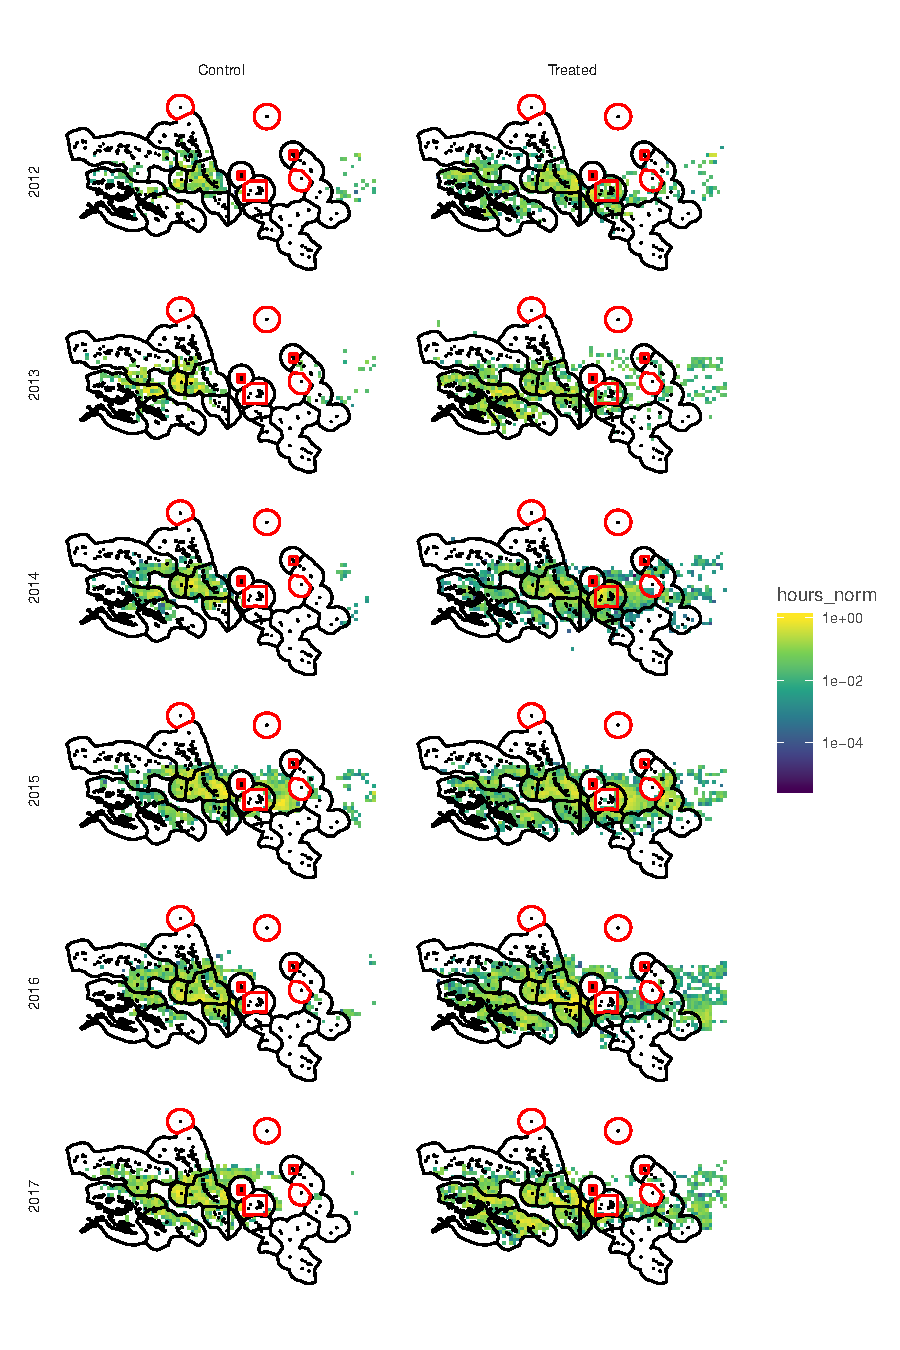
\includegraphics{C:/Users/JC/Documents/GitHub/MPA_displacement/docs/Manuscript_files/figure-latex/unnamed-chunk-14-1.pdf}
\caption{\label{fig:unnamed-chunk-14}\label{fig:redist_trend_ps}Monthly
relative allocation of fishing effort by PIPA-fishing vessels before and
after PIPA for 9 EEZs, PIPA, the high seas and `other EEZs'.}
\end{figure}

\begin{figure}
\centering
\includegraphics{C:/Users/JC/Documents/GitHub/MPA_displacement/docs/Manuscript_files/figure-latex/unnamed-chunk-17-1.pdf}
\caption{\label{fig:unnamed-chunk-17}\label{fig:map_change_ps}Spatial
representation of the mean change in the monthly allocation of fishing
effort for purse seiners.}
\end{figure}

\begin{figure}
\centering
\includegraphics{C:/Users/JC/Documents/GitHub/MPA_displacement/docs/Manuscript_files/figure-latex/unnamed-chunk-18-1.pdf}
\caption{\label{fig:unnamed-chunk-18}\label{fig:map_change_ps}Spatial
representation of the mean change in the monthly allocation of fishing
effort for longliners. \textbf{This are preliminar results, contingent
on the spatial analysis currently being run}}
\end{figure}

\begin{table}[!htbp] \centering 
  \caption{\label{tab:disp_mod}Change in the relative allocation of fishing hours by purse seiners for each region. Asterisks indicate significance levels. Numbers in parenthesis represent heteroskedastic-robust standard errors.} 
  \label{} 
\begin{tabular}{@{\extracolsep{5pt}}lc} 
\\[-1.8ex]\hline 
\hline \\[-1.8ex] 
 & \multicolumn{1}{c}{\textit{Dependent variable:}} \\ 
\cline{2-2} 
\\[-1.8ex] & h\_prop \\ 
\hline \\[-1.8ex] 
 post & $-$0.085$^{***}$ (0.018) \\ 
  countryKIR & 0.251$^{***}$ (0.036) \\ 
  countryHS & $-$0.089$^{***}$ (0.018) \\ 
  countryCOK & $-$0.085$^{***}$ (0.018) \\ 
  countryFSM & $-$0.034 (0.021) \\ 
  countryMHL & $-$0.063$^{***}$ (0.019) \\ 
  countryNRU & $-$0.039$^{**}$ (0.020) \\ 
  countryPNG & 0.098$^{***}$ (0.034) \\ 
  countrySLB & $-$0.023 (0.026) \\ 
  countryTKL & $-$0.072$^{***}$ (0.018) \\ 
  countryTUV & $-$0.024 (0.021) \\ 
  countryothers & 0.016 (0.021) \\ 
  post:countryKIR & 0.113$^{**}$ (0.045) \\ 
  post:countryHS & 0.085$^{***}$ (0.018) \\ 
  post:countryCOK & 0.089$^{***}$ (0.018) \\ 
  post:countryFSM & 0.091$^{***}$ (0.025) \\ 
  post:countryMHL & 0.080$^{***}$ (0.021) \\ 
  post:countryNRU & 0.087$^{***}$ (0.021) \\ 
  post:countryPNG & $-$0.015 (0.037) \\ 
  post:countrySLB & 0.107$^{***}$ (0.031) \\ 
  post:countryTKL & 0.087$^{***}$ (0.019) \\ 
  post:countryTUV & 0.100$^{***}$ (0.025) \\ 
  post:countryothers & 0.201$^{***}$ (0.028) \\ 
  Constant & 0.089$^{***}$ (0.018) \\ 
 \hline \\[-1.8ex] 
Observations & 864 \\ 
R$^{2}$ & 0.557 \\ 
\hline 
\hline \\[-1.8ex] 
\textit{Note:}  & \multicolumn{1}{r}{$^{*}$p$<$0.1; $^{**}$p$<$0.05; $^{***}$p$<$0.01} \\ 
\end{tabular} 
\end{table}

\clearpage

\section{Discusion}\label{discusion}

Our findings provide interesting insights into the effect that LSMPAs
can have on vessel behavior and the redistribution of fishing effort.
These collection of results shows that the implementation of PIPA caused
treated vessels to reduce their fishing hours, and that this effect is
greater for purse seiners than longliners. Even though treated vessels
fish less, their relative allocation of fishing hours increased for all
other fishing grounds. This does not imply that there is more fishing
effort exerted by treated vessels, but rather that each region receives
a greater portion of the post-PIPA fishing effort of these same vessels,
which is lower than pre-PIPA levels. In this section we discuss the
implications of vessel-level reductions in fishing effort and the
increase in relative allocation of the remaining effort through space.
We also provide plausible explanations as to why purse seiners seem to
be more reactive to the spatial closure.

A major shortcoming of our analyses is that we do not observe catches or
revenues, which ultimately are the factors that guide the decision
making process of profit-maximizing agents. Therefore, it is difficult
to know whether the reduction in fishing effort represents a positive or
negative impact. A decrease in fishing effort is associated to an
increase in catches (and therefore greater CPUE) only when the entire
fleet does it, and if previous levels of effort were greater than
\(F_{MEY}\) (\emph{i.e.} the effort that would yield the maximum
economic yield). Therefore, it is plausible that the reduction of
fishing hours is not done by choice, but rather results from fishers
having to increase search time. Upon being relocated, fishers may not
identify the best fishing grounds as easily as before, and therefore
invest a greater proportion of their time searching for their catch.
Further analysis of temporal trends in non-fishing hours, as well as
distance traveled should provide us with insights as to why fishers
reduced fishing hours.

Previous studies on insular environments suggest that vessels move to
distant places, which might be translated as increased costs
\citep{stevenson_2013}. Nevertheless, they do not use counterfactuals
that could help account for system- or fleet-level changes that occur
through time. Others have used similar satellite-tracking systems to
show that fishing effort accumulates near the edges of spatial closures,
yielding greater catches \citep{murawski_2005}. Yet, these vessel tracks
do not cover the pre-reserve period, making it difficult identify the
contribution of spatial closures to the observed spatial distribution of
fishing vessels. Recent work by \citet{elahi_2018} identified that total
fishing effort in a focal region where a short-term MPA was implemented
showed little change, likely indicating that fishers redistributed
fishing effort to compensate for the reduction in available space. Our
data is assembled in a similar way, with fishing positions before and
after the implementation of PIPA and vessels grouped into treated and
control groups. Our BACI design, along with our
difference-in-differences analysis allows us to make causal inferences
about the effect that large scale marine protected areas have on fishing
effort.

The different responses observed between purse seiners and longliners
might have two possible explanations. It is likely that PIPA did not
contain habitat that longliners would consider optimal. Therefore, the
sporadic fishing events that occurred there are of little importance to
the fleet, and it is unlikely that the implementation of PIPA has an
effect on them. Alternatively, the differences may be due to the nature
of each fishing gear. Purse seiners are often constrained by seafloor
and termocline depth, and have a smaller spatial footprint
\citep{kroodsma_2018}. Tuna purse seiners are known to have greater
proportion of null sets (\emph{i.e.} where purse seines effectively cast
their nets, but no catch is obtained) during El Niño years, where the
termocline deepens in the Eastern Pacific \citep{dreyfusleon_2015}. On
the other hand, longliners may be more flexible as to where they can
deploy their longlines. \citet{ortuocrespo_2018} evaluated the
ecological niche of the pelagic longline fleet, and suggest that the
fleet may be under-utilizing the ocean, meaning that they can easily
redistribute elsewhere.

Our work suggests that the implementation of LSMPAs can have important
implications for purse seiners, and less so for longliners. We also show
that fishing effort is redistributed to areas close by. Future
management interventions that aim to close large portion of the oceans
should consider how fishing effort will change in space and through
time, and the ecological implications of this redistribution to ensure
that fishing effort is not just displaced elsewhere, leading to
overfishing in adjacent waters.

\clearpage

\section{Appendix}\label{appendix}

\begin{table}[!htbp] \centering 
  \caption{\label{tab:purse_old}Fishing hours from GFW for purse seiners (n = 106; 38 control, 68 treatment). Asterisks indicate significance levels. Numbers in parenthesis represent heteroskedastic-robuste standard errors.} 
  \label{} 
\begin{tabular}{@{\extracolsep{5pt}}lcccc} 
\\[-1.8ex]\hline 
\hline \\[-1.8ex] 
 & \multicolumn{4}{c}{\textit{Dependent variable:}} \\ 
\cline{2-5} 
\\[-1.8ex] & \multicolumn{4}{c}{hours} \\ 
\\[-1.8ex] & (1) & (2) & (3) & (4)\\ 
\hline \\[-1.8ex] 
 post & 95.087$^{***}$ & 99.232$^{***}$ & 146.372$^{***}$ & 119.222$^{***}$ \\ 
  & (5.877) & (5.453) & (6.926) & (6.717) \\ 
  & & & & \\ 
 treated & $-$6.575 & $-$5.597 & $-$6.050 & 2.925 \\ 
  & (4.985) & (4.564) & (4.095) & (5.052) \\ 
  & & & & \\ 
 post:treated & $-$16.457$^{**}$ & $-$16.739$^{***}$ & $-$14.748$^{**}$ & $-$16.231$^{**}$ \\ 
  & (6.856) & (6.460) & (6.152) & (6.692) \\ 
  & & & & \\ 
 Constant & 59.490$^{***}$ & 65.485$^{***}$ & 36.643$^{***}$ & 53.138$^{***}$ \\ 
  & (4.422) & (6.132) & (6.462) & (10.394) \\ 
  & & & & \\ 
\hline \\[-1.8ex] 
Month FE & No & Yes & Yes & Yes \\ 
Year FE & No & No & Yes & Yes \\ 
Flag FE & No & No & No & Yes \\ 
Observations & 3,867 & 3,867 & 3,867 & 3,481 \\ 
R$^{2}$ & 0.171 & 0.243 & 0.301 & 0.320 \\ 
\hline 
\hline \\[-1.8ex] 
\textit{Note:}  & \multicolumn{4}{r}{$^{*}$p$<$0.1; $^{**}$p$<$0.05; $^{***}$p$<$0.01} \\ 
\end{tabular} 
\end{table}

\begin{table}[!htbp] \centering 
  \caption{\label{tab:long}Fishing hours from GFW for longliners (n = 203; 88 control, 115 treatment).. Asterisks indicate significance levels. Numbers in parenthesis represent heteroskedastic-robuste standard errors.} 
  \label{} 
\begin{tabular}{@{\extracolsep{5pt}}lcccc} 
\\[-1.8ex]\hline 
\hline \\[-1.8ex] 
 & \multicolumn{4}{c}{\textit{Dependent variable:}} \\ 
\cline{2-5} 
\\[-1.8ex] & \multicolumn{4}{c}{hours} \\ 
\\[-1.8ex] & (1) & (2) & (3) & (4)\\ 
\hline \\[-1.8ex] 
 post & $-$11.929 & $-$6.968 & 8.201 & 17.751$^{*}$ \\ 
  & (7.969) & (7.975) & (11.119) & (10.388) \\ 
  & & & & \\ 
 treated & 70.142$^{***}$ & 72.314$^{***}$ & 72.243$^{***}$ & 13.875$^{*}$ \\ 
  & (7.200) & (7.200) & (7.283) & (7.992) \\ 
  & & & & \\ 
 post:treated & $-$9.851 & $-$12.290 & $-$13.287 & $-$14.750 \\ 
  & (9.294) & (9.262) & (9.344) & (9.569) \\ 
  & & & & \\ 
 Constant & 474.478$^{***}$ & 449.960$^{***}$ & 449.666$^{***}$ & 429.919$^{***}$ \\ 
  & (6.328) & (9.440) & (11.122) & (27.606) \\ 
  & & & & \\ 
\hline \\[-1.8ex] 
Month FE & No & Yes & Yes & Yes \\ 
Year FE & No & No & Yes & Yes \\ 
Flag FE & No & No & No & Yes \\ 
Observations & 9,460 & 9,460 & 9,460 & 8,269 \\ 
R$^{2}$ & 0.027 & 0.041 & 0.042 & 0.094 \\ 
\hline 
\hline \\[-1.8ex] 
\textit{Note:}  & \multicolumn{4}{r}{$^{*}$p$<$0.1; $^{**}$p$<$0.05; $^{***}$p$<$0.01} \\ 
\end{tabular} 
\end{table}

\clearpage

\bibliography{references.bib}


\end{document}
